
\centering


\tikzset{every picture/.style={line width=0.75pt}} %set default line width to 0.75pt        

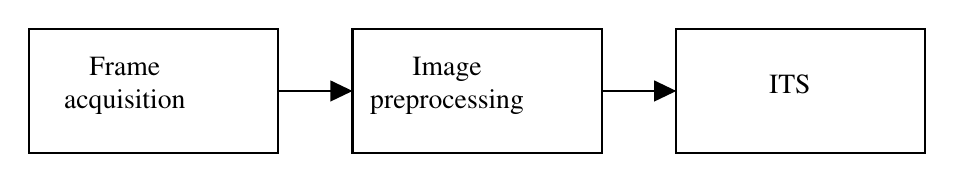
\begin{tikzpicture}[x=0.75pt,y=0.75pt,yscale=-1.2,xscale=1.2]
%uncomment if require: \path (0,300); %set diagram left start at 0, and has height of 300

%Shape: Rectangle [id:dp5311967622096787] 
\draw  [fill={rgb, 255:red, 255; green, 255; blue, 255 }  ,fill opacity=1 ] (20,20) -- (120,20) -- (120,70) -- (20,70) -- cycle ;
%Shape: Rectangle [id:dp07593828947048697] 
\draw  [fill={rgb, 255:red, 255; green, 255; blue, 255 }  ,fill opacity=1 ] (150,20) -- (250,20) -- (250,70) -- (150,70) -- cycle ;
%Shape: Rectangle [id:dp1321828393456428] 
\draw  [fill={rgb, 255:red, 255; green, 255; blue, 255 }  ,fill opacity=1 ] (280,20) -- (380,20) -- (380,70) -- (280,70) -- cycle ;
%Straight Lines [id:da24611526462953326] 
\draw    (120,45) -- (147,45) ;
\draw [shift={(150,45)}, rotate = 180] [fill={rgb, 255:red, 0; green, 0; blue, 0 }  ][line width=0.08]  [draw opacity=0] (8.93,-4.29) -- (0,0) -- (8.93,4.29) -- cycle    ;
%Straight Lines [id:da283033721708871] 
\draw    (250,45) -- (277,45) ;
\draw [shift={(280,45)}, rotate = 180] [fill={rgb, 255:red, 0; green, 0; blue, 0 }  ][line width=0.08]  [draw opacity=0] (8.93,-4.29) -- (0,0) -- (8.93,4.29) -- cycle    ;

% Text Node
\draw (30.67,30.00) node [anchor=north west][inner sep=0.75pt]   [align=left] {\begin{minipage}[lt]{48.000000pt}\setlength\topsep{0pt}
\begin{center}
{\fontfamily{ptm}\selectfont Frame}\\{\fontfamily{ptm}\selectfont  acquisition}
\end{center}

\end{minipage}};
% Text Node
\draw (152,30) node [anchor=north west][inner sep=0.75pt]   [align=left] {\begin{minipage}[lt]{62.482752pt}\setlength\topsep{0pt}
\begin{center}
{\fontfamily{ptm}\selectfont Image}\\{\fontfamily{ptm}\selectfont  preprocessing}
\end{center}

\end{minipage}};
% Text Node
\draw (316,37) node [anchor=north west][inner sep=0.75pt]   [align=left] {{\fontfamily{ptm}\selectfont ITS}};


\end{tikzpicture}
